\begin{frame}[t]{Office pre-trajectories: drafted offices}
    \centering
    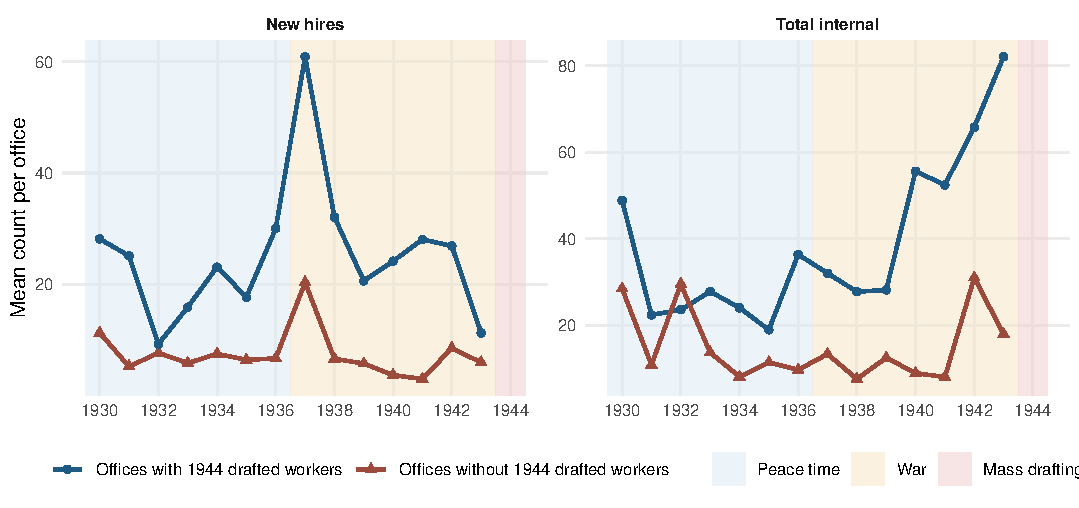
\includegraphics[width=0.88\textwidth]{Results/draft1944_pre_draft_trajectories/office_raw_trajectory_total_internal_new_hires.pdf}
    \vspace{1mm}
    {\tiny Descriptive office-level 1930--1943 trajectories, grouped by whether the office contains any worker later marked drafted in the 1944 TokyoTo directory. Outcomes exclude those eventual draftees.}
\end{frame}

\begin{frame}[t]{Pre-trends: adjusted office differences}
    \tiny
    \centering
    \begin{threeparttable}
    \begin{tabular}{lcccccc}
        \toprule
        & \multicolumn{6}{c}{\textit{Adjusted difference: offices with 1944 drafted workers}} \\
        \cmidrule(lr){2-7}
        & 1930 & 1933 & 1936 & 1939 & 1941 & 1943 \\
        \midrule
        Total internal & 16.929 & 12.029 & 12.760$^{*}$ & 11.945$^{**}$ & 42.652$^{***}$ & 58.037$^{***}$ \\
 & (19.476) & (8.022) & (7.512) & (5.707) & (11.499) & (10.456) \\
        Retention & -4.544$^{*}$ & 0.450 & 9.348 & 2.730 & 22.992$^{***}$ & 31.079$^{***}$ \\
 & (2.353) & (0.478) & (6.298) & (1.889) & (7.217) & (8.077) \\
        New hires & 13.382$^{*}$ & 8.536$^{*}$ & 12.197$^{*}$ & 9.128$^{**}$ & 21.595$^{***}$ & 3.225$^{**}$ \\
 & (8.047) & (4.913) & (7.005) & (4.503) & (6.647) & (1.636) \\
        \midrule
        Future-drafted offices & \multicolumn{6}{c}{118} \\
        Future drafted workers & \multicolumn{6}{c}{554} \\
        Baseline male employment (log) & \multicolumn{6}{c}{Yes} \\
        \bottomrule
    \end{tabular}
    \begin{tablenotes}[flushleft]
        \tiny
        \item \textit{Notes:} Separate year-by-year office-level OLS differences relative to offices without future draftees. Outcomes exclude workers later marked drafted in the 1944 TokyoTo directory. The table reports selected years from the 1930--1943 trajectory window. Specifications control for log cumulative male baseline employment. Standard errors clustered by office in parentheses. $^{***}p<0.01$, $^{**}p<0.05$, $^{*}p<0.1$.
    \end{tablenotes}
    \end{threeparttable}
\end{frame}

\begin{frame}[t]{Within-section pre-trend: cell size}
    \hypertarget{app:pretrend-workers-plot}{}
    \centering
    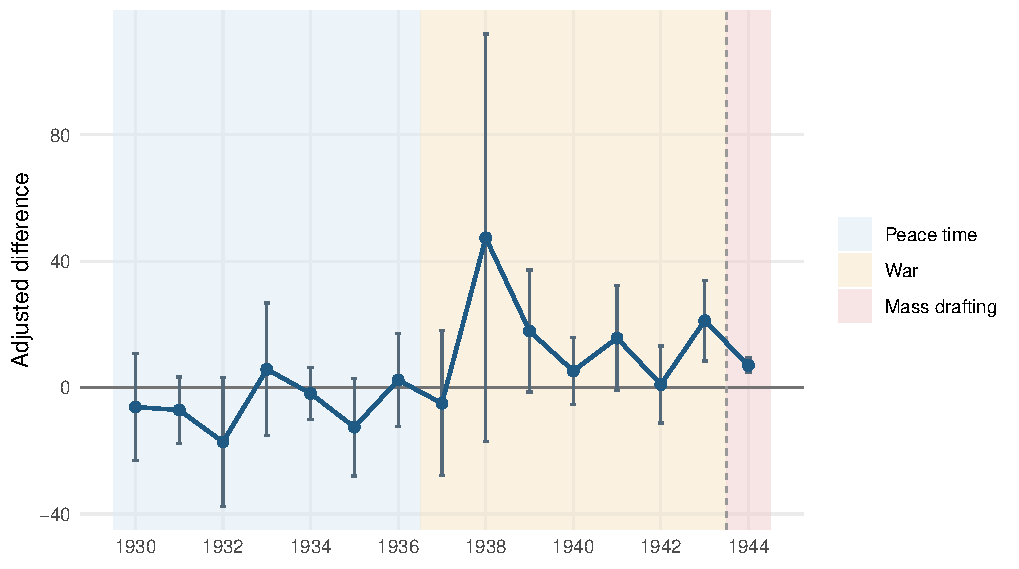
\includegraphics[width=0.84\textwidth]{Results/draft1944_pre_draft_trajectories/within_section_pretrend_workers.pdf}
    \vspace{1mm}
    \parbox{0.9\textwidth}{\centering\tiny Unit: section $\times$ team $\times$ occupation. Conditional on section and position; controls for log cumulative male baseline. Bars show 95\% confidence intervals.}
\end{frame}

\begin{frame}[t]{Within-section pre-trend: cell size DID}
    \hypertarget{app:pretrend-workers-table}{}
    \scriptsize
    \centering
    \begin{threeparttable}
    \begin{tabular}{lcc}
        \toprule
        & Cell + year FE & Section/position + year FE \\
        \midrule
        Future drafted cell $\times$ War & 29.468$^{***}$ & 16.411$^{***}$ \\
        & (7.660) & (5.901) \\
        Future drafted cell $\times$ Mass drafting & 1.568 & 4.114$^{***}$ \\
        & (9.395) & (1.303) \\
        \midrule
        Observations & 6,776 & 10,108 \\
        Cells & \multicolumn{2}{c}{5,419} \\
        Sections & \multicolumn{2}{c}{982} \\
        Baseline male employment (log) & Yes & Yes \\
        \bottomrule
    \end{tabular}
    \begin{tablenotes}[flushleft]
        \tiny
        \item \textit{Notes:} Outcome is measured in the section $\times$ team $\times$ occupation cell, excluding workers later marked drafted in the 1944 TokyoTo directory. Treatment is whether the cell contains any 1944 male draftee. Coefficients are DID estimates relative to peace time. Peace time, 1930--1936, is the omitted period; War is 1937--1943; Mass drafting is 1944. Standard errors clustered by section in parentheses. $^{***}p<0.01$, $^{**}p<0.05$, $^{*}p<0.1$.
    \end{tablenotes}
    \end{threeparttable}
\end{frame}

\begin{frame}[t]{Within-section pre-trend: internal flows}
    \hypertarget{app:pretrend-internal-plot}{}
    \centering
    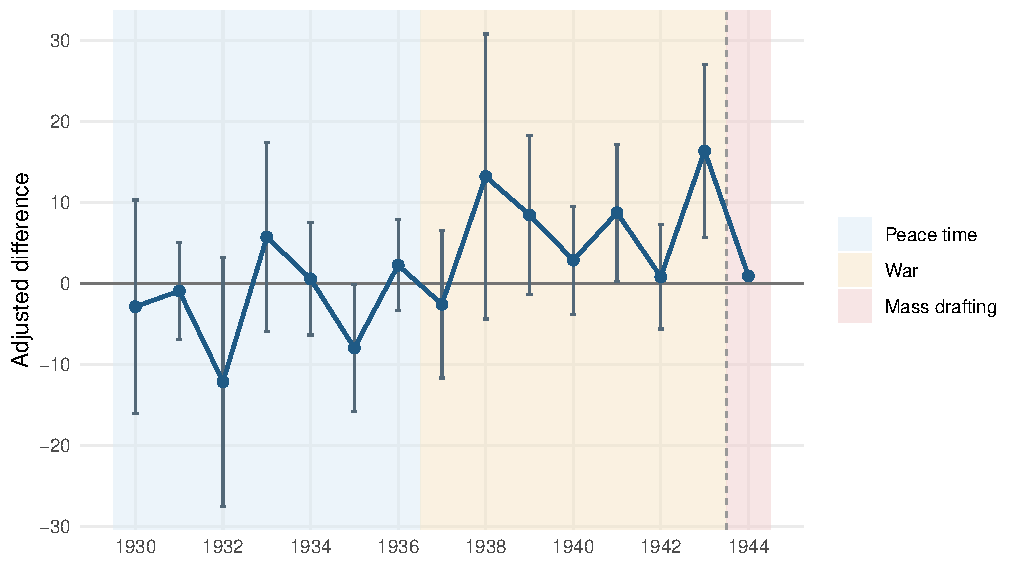
\includegraphics[width=0.84\textwidth]{Results/draft1944_pre_draft_trajectories/within_section_pretrend_internal.pdf}
    \vspace{1mm}
    \parbox{0.9\textwidth}{\centering\tiny Unit: section $\times$ team $\times$ occupation. Conditional on section and position; controls for log cumulative male baseline. Bars show 95\% confidence intervals.}
\end{frame}

\begin{frame}[t]{Within-section pre-trend: internal flows DID}
    \hypertarget{app:pretrend-internal-table}{}
    \scriptsize
    \centering
    \begin{threeparttable}
    \begin{tabular}{lcc}
        \toprule
        & Cell + year FE & Section/position + year FE \\
        \midrule
        Future drafted cell $\times$ War & 12.967$^{***}$ & 9.880$^{***}$ \\
        & (3.938) & (2.964) \\
        Future drafted cell $\times$ Mass drafting & -1.042 & 0.117 \\
        & (4.310) & (0.411) \\
        \midrule
        Observations & 6,776 & 10,108 \\
        Cells & \multicolumn{2}{c}{5,419} \\
        Sections & \multicolumn{2}{c}{982} \\
        Baseline male employment (log) & Yes & Yes \\
        \bottomrule
    \end{tabular}
    \begin{tablenotes}[flushleft]
        \tiny
        \item \textit{Notes:} Outcome is measured in the section $\times$ team $\times$ occupation cell, excluding workers later marked drafted in the 1944 TokyoTo directory. Treatment is whether the cell contains any 1944 male draftee. Coefficients are DID estimates relative to peace time. Peace time, 1930--1936, is the omitted period; War is 1937--1943; Mass drafting is 1944. Standard errors clustered by section in parentheses. $^{***}p<0.01$, $^{**}p<0.05$, $^{*}p<0.1$.
    \end{tablenotes}
    \end{threeparttable}
\end{frame}

\begin{frame}[t]{Within-section pre-trend: retention}
    \hypertarget{app:pretrend-retention-plot}{}
    \centering
    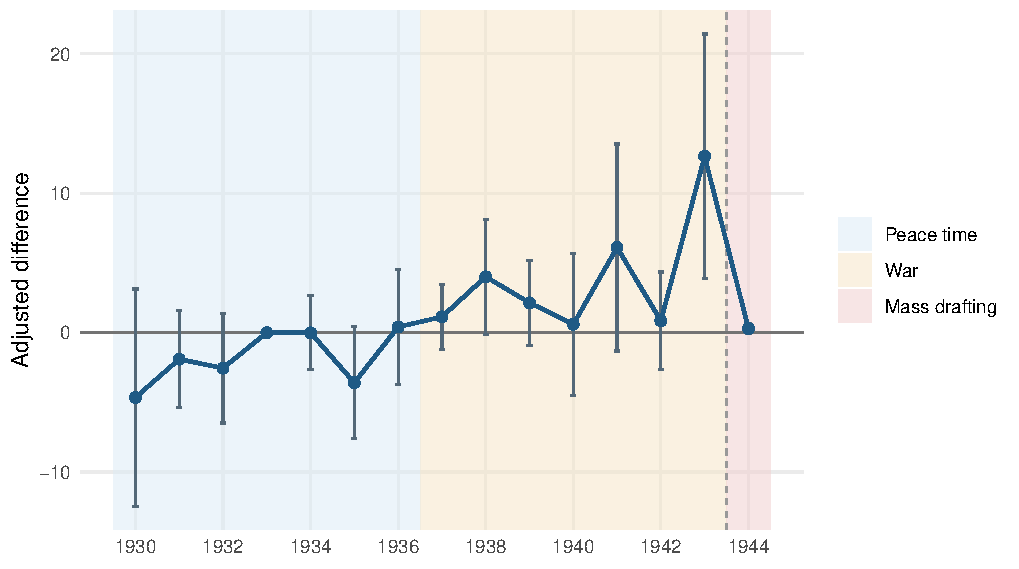
\includegraphics[width=0.84\textwidth]{Results/draft1944_pre_draft_trajectories/within_section_pretrend_retention.pdf}
    \vspace{1mm}
    \parbox{0.9\textwidth}{\centering\tiny Unit: section $\times$ team $\times$ occupation. Conditional on section and position; controls for log cumulative male baseline. Bars show 95\% confidence intervals.}
\end{frame}

\begin{frame}[t]{Within-section pre-trend: retention DID}
    \hypertarget{app:pretrend-retention-table}{}
    \scriptsize
    \centering
    \begin{threeparttable}
    \begin{tabular}{lcc}
        \toprule
        & Cell + year FE & Section/position + year FE \\
        \midrule
        Future drafted cell $\times$ War & 8.373$^{***}$ & 6.754$^{***}$ \\
        & (2.520) & (1.835) \\
        Future drafted cell $\times$ Mass drafting & 2.219$^{**}$ & 0.219 \\
        & (1.053) & (0.213) \\
        \midrule
        Observations & 6,776 & 10,108 \\
        Cells & \multicolumn{2}{c}{5,419} \\
        Sections & \multicolumn{2}{c}{982} \\
        Baseline male employment (log) & Yes & Yes \\
        \bottomrule
    \end{tabular}
    \begin{tablenotes}[flushleft]
        \tiny
        \item \textit{Notes:} Outcome is measured in the section $\times$ team $\times$ occupation cell, excluding workers later marked drafted in the 1944 TokyoTo directory. Treatment is whether the cell contains any 1944 male draftee. Coefficients are DID estimates relative to peace time. Peace time, 1930--1936, is the omitted period; War is 1937--1943; Mass drafting is 1944. Standard errors clustered by section in parentheses. $^{***}p<0.01$, $^{**}p<0.05$, $^{*}p<0.1$.
    \end{tablenotes}
    \end{threeparttable}
\end{frame}

\begin{frame}[t]{Within-section pre-trend: same-dept transfers}
    \hypertarget{app:pretrend-same-dept-plot}{}
    \centering
    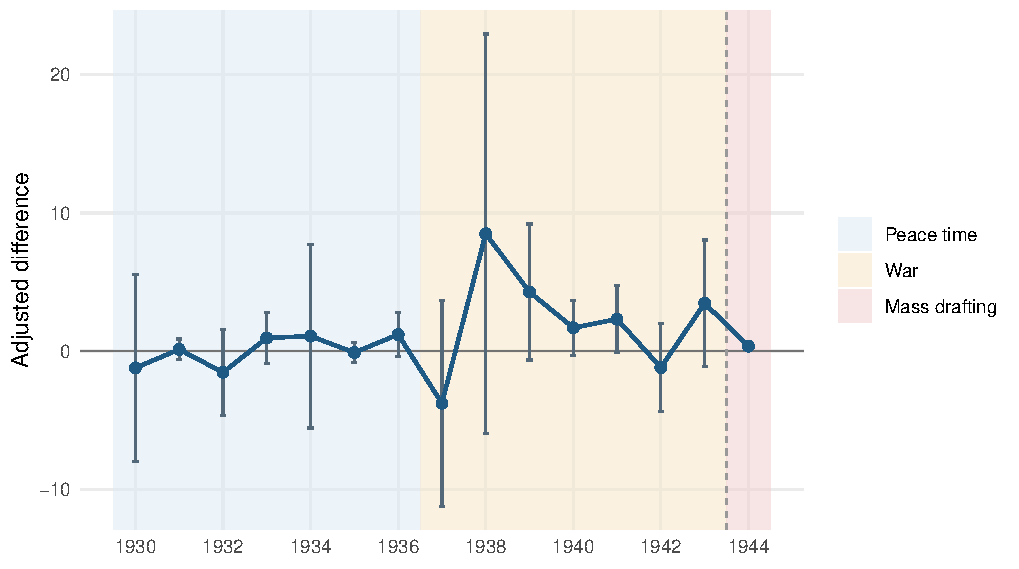
\includegraphics[width=0.84\textwidth]{Results/draft1944_pre_draft_trajectories/within_section_pretrend_same_dept.pdf}
    \vspace{1mm}
    \parbox{0.9\textwidth}{\centering\tiny Unit: section $\times$ team $\times$ occupation. Conditional on section and position; controls for log cumulative male baseline. Bars show 95\% confidence intervals.}
\end{frame}

\begin{frame}[t]{Within-section pre-trend: same-dept transfers DID}
    \hypertarget{app:pretrend-same-dept-table}{}
    \scriptsize
    \centering
    \begin{threeparttable}
    \begin{tabular}{lcc}
        \toprule
        & Cell + year FE & Section/position + year FE \\
        \midrule
        Future drafted cell $\times$ War & 2.849 & 2.759$^{*}$ \\
        & (1.731) & (1.416) \\
        Future drafted cell $\times$ Mass drafting & -0.722 & -0.237 \\
        & (1.231) & (0.215) \\
        \midrule
        Observations & 6,776 & 10,108 \\
        Cells & \multicolumn{2}{c}{5,419} \\
        Sections & \multicolumn{2}{c}{982} \\
        Baseline male employment (log) & Yes & Yes \\
        \bottomrule
    \end{tabular}
    \begin{tablenotes}[flushleft]
        \tiny
        \item \textit{Notes:} Outcome is measured in the section $\times$ team $\times$ occupation cell, excluding workers later marked drafted in the 1944 TokyoTo directory. Treatment is whether the cell contains any 1944 male draftee. Coefficients are DID estimates relative to peace time. Peace time, 1930--1936, is the omitted period; War is 1937--1943; Mass drafting is 1944. Standard errors clustered by section in parentheses. $^{***}p<0.01$, $^{**}p<0.05$, $^{*}p<0.1$.
    \end{tablenotes}
    \end{threeparttable}
\end{frame}

\begin{frame}[t]{Within-section pre-trend: diff.-dept transfers}
    \hypertarget{app:pretrend-diff-dept-plot}{}
    \centering
    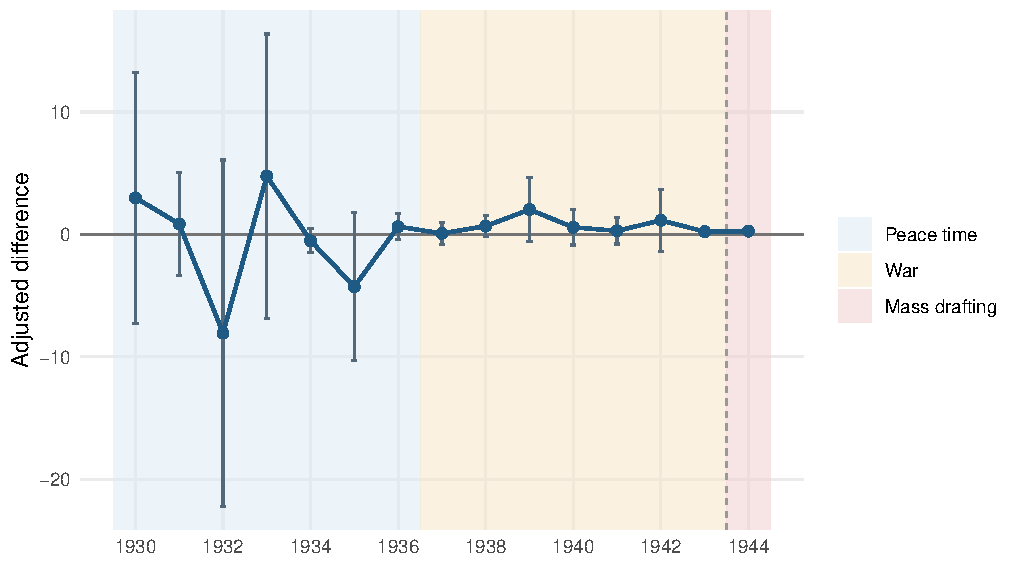
\includegraphics[width=0.84\textwidth]{Results/draft1944_pre_draft_trajectories/within_section_pretrend_diff_dept.pdf}
    \vspace{1mm}
    \parbox{0.9\textwidth}{\centering\tiny Unit: section $\times$ team $\times$ occupation. Conditional on section and position; controls for log cumulative male baseline. Bars show 95\% confidence intervals.}
\end{frame}

\begin{frame}[t]{Within-section pre-trend: diff.-dept transfers DID}
    \hypertarget{app:pretrend-diff-dept-table}{}
    \scriptsize
    \centering
    \begin{threeparttable}
    \begin{tabular}{lcc}
        \toprule
        & Cell + year FE & Section/position + year FE \\
        \midrule
        Future drafted cell $\times$ War & 1.744$^{***}$ & 0.366 \\
        & (0.648) & (0.421) \\
        Future drafted cell $\times$ Mass drafting & -2.539 & 0.135 \\
        & (3.512) & (0.176) \\
        \midrule
        Observations & 6,776 & 10,108 \\
        Cells & \multicolumn{2}{c}{5,419} \\
        Sections & \multicolumn{2}{c}{982} \\
        Baseline male employment (log) & Yes & Yes \\
        \bottomrule
    \end{tabular}
    \begin{tablenotes}[flushleft]
        \tiny
        \item \textit{Notes:} Outcome is measured in the section $\times$ team $\times$ occupation cell, excluding workers later marked drafted in the 1944 TokyoTo directory. Treatment is whether the cell contains any 1944 male draftee. Coefficients are DID estimates relative to peace time. Peace time, 1930--1936, is the omitted period; War is 1937--1943; Mass drafting is 1944. Standard errors clustered by section in parentheses. $^{***}p<0.01$, $^{**}p<0.05$, $^{*}p<0.1$.
    \end{tablenotes}
    \end{threeparttable}
\end{frame}

\begin{frame}[t]{Within-section pre-trend: new hires}
    \hypertarget{app:pretrend-new-hires-plot}{}
    \centering
    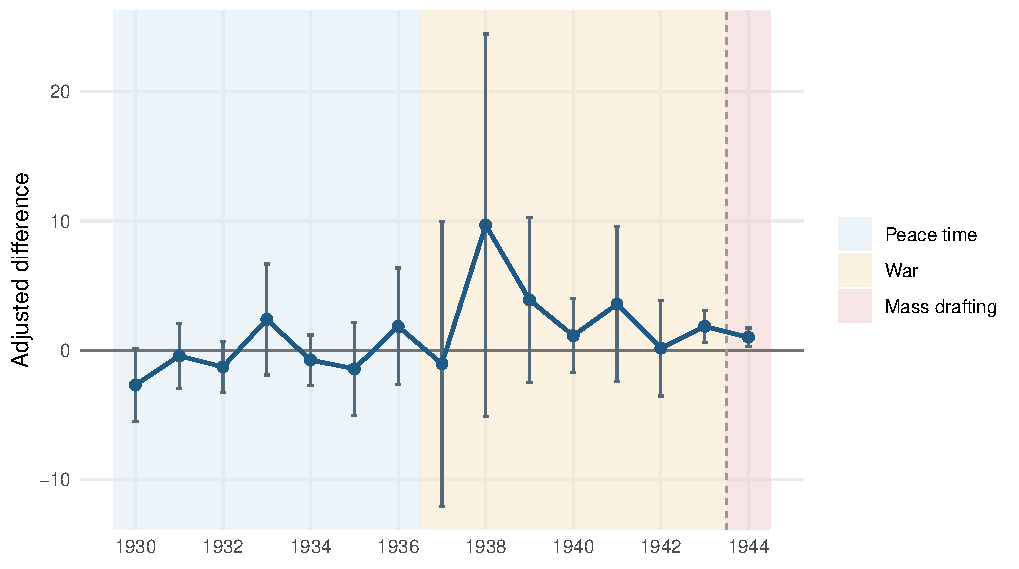
\includegraphics[width=0.84\textwidth]{Results/draft1944_pre_draft_trajectories/within_section_pretrend_new_hires.pdf}
    \vspace{1mm}
    \parbox{0.9\textwidth}{\centering\tiny Unit: section $\times$ team $\times$ occupation. Conditional on section and position; controls for log cumulative male baseline. Bars show 95\% confidence intervals.}
\end{frame}

\begin{frame}[t]{Within-section pre-trend: new hires DID}
    \hypertarget{app:pretrend-new-hires-table}{}
    \scriptsize
    \centering
    \begin{threeparttable}
    \begin{tabular}{lcc}
        \toprule
        & Cell + year FE & Section/position + year FE \\
        \midrule
        Future drafted cell $\times$ War & 7.137$^{**}$ & 2.861 \\
        & (2.908) & (1.741) \\
        Future drafted cell $\times$ Mass drafting & 2.037 & -0.223 \\
        & (2.395) & (0.384) \\
        \midrule
        Observations & 6,776 & 10,108 \\
        Cells & \multicolumn{2}{c}{5,419} \\
        Sections & \multicolumn{2}{c}{982} \\
        Baseline male employment (log) & Yes & Yes \\
        \bottomrule
    \end{tabular}
    \begin{tablenotes}[flushleft]
        \tiny
        \item \textit{Notes:} Outcome is measured in the section $\times$ team $\times$ occupation cell, excluding workers later marked drafted in the 1944 TokyoTo directory. Treatment is whether the cell contains any 1944 male draftee. Coefficients are DID estimates relative to peace time. Peace time, 1930--1936, is the omitted period; War is 1937--1943; Mass drafting is 1944. Standard errors clustered by section in parentheses. $^{***}p<0.01$, $^{**}p<0.05$, $^{*}p<0.1$.
    \end{tablenotes}
    \end{threeparttable}
\end{frame}

\begin{frame}[t]{Draft intensity: internal transfers event study}
    \hypertarget{app:intensity-internal-plot}{}
    \centering
    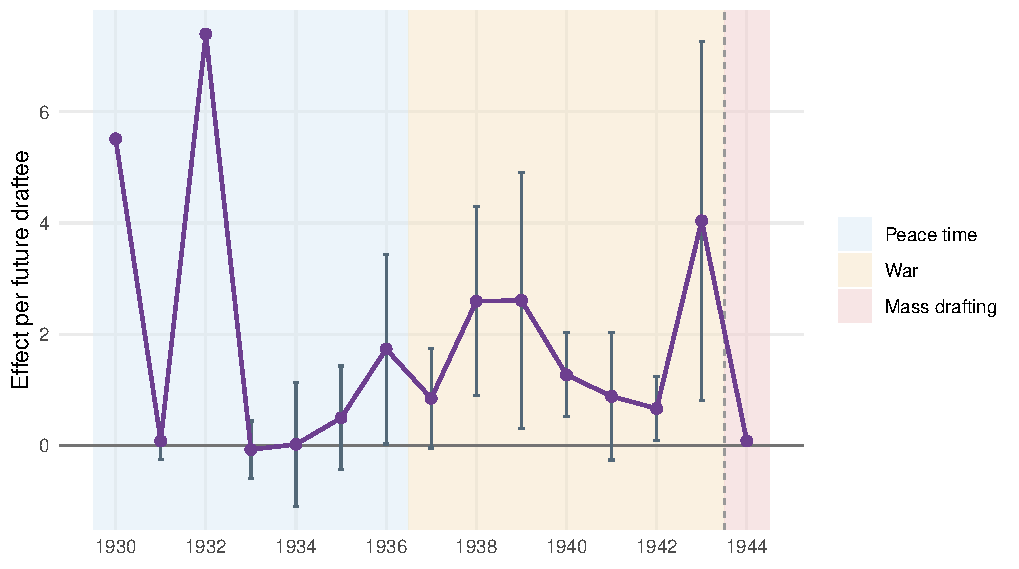
\includegraphics[width=0.84\textwidth]{Results/draft1944_pre_draft_trajectories/draft_intensity_treatment_internal.pdf}
    \vspace{1mm}
    \parbox{0.9\textwidth}{\centering\tiny Outcome: total internal arrivals; treatment: number of future draftees. Conditional on section and occupation; controls for log cumulative male baseline. Bars show 95\% confidence intervals.}
\end{frame}

\begin{frame}[t]{Draft intensity: internal transfers event study DID}
    \hypertarget{app:intensity-internal-table}{}
    \scriptsize
    \centering
    \begin{threeparttable}
    \begin{tabular}{lccc}
        \toprule
        & Section + occ. + year FE & No section FE & No occ. FE \\
        \midrule
        No. future drafted $\times$ War & 2.098$^{***}$ & 2.320$^{***}$ & 2.060$^{***}$ \\
        & (0.678) & (0.812) & (0.654) \\
        No. future drafted $\times$ Mass drafting & -0.120 & 0.004 & 0.001 \\
        & (0.152) & (0.133) & (0.058) \\
        \midrule
        Observations & 936 & 988 & 938 \\
        Sections clustered & \multicolumn{3}{c}{173} \\
        Baseline male employment (log) & Yes & Yes & Yes \\
        \bottomrule
    \end{tabular}
    \begin{tablenotes}[flushleft]
        \tiny
        \item \textit{Notes:} Outcome is measured in the section $\times$ team $\times$ occupation cell. Treatment is the number of male workers drafted in 1944 from the same future cell. Peace time, 1930--1936, is the omitted period; War is 1937--1943; Mass drafting is 1944. Standard errors clustered by section in parentheses. $^{***}p<0.01$, $^{**}p<0.05$, $^{*}p<0.1$.
    \end{tablenotes}
    \end{threeparttable}
\end{frame}

\begin{frame}[t]{Draft intensity: external hires event study}
    \hypertarget{app:intensity-new-hires-plot}{}
    \centering
    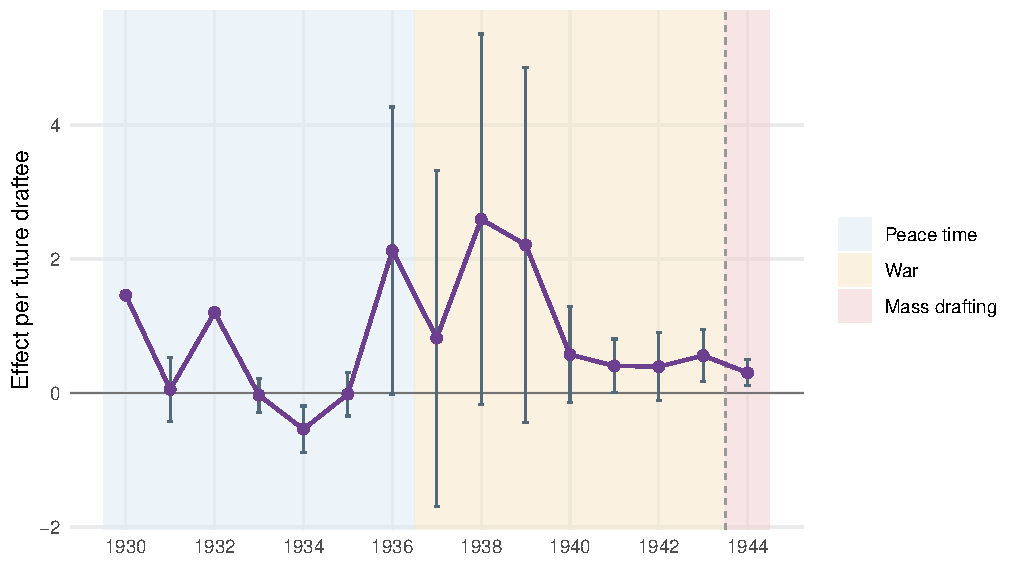
\includegraphics[width=0.84\textwidth]{Results/draft1944_pre_draft_trajectories/draft_intensity_treatment_new_hires.pdf}
    \vspace{1mm}
    \parbox{0.9\textwidth}{\centering\tiny Outcome: external new hires; treatment: number of future draftees. Conditional on section and occupation; controls for log cumulative male baseline. Bars show 95\% confidence intervals.}
\end{frame}

\begin{frame}[t]{Draft intensity: external hires event study DID}
    \hypertarget{app:intensity-new-hires-table}{}
    \scriptsize
    \centering
    \begin{threeparttable}
    \begin{tabular}{lccc}
        \toprule
        & Section + occ. + year FE & No section FE & No occ. FE \\
        \midrule
        No. future drafted $\times$ War & 0.924 & 0.903$^{*}$ & 1.014$^{*}$ \\
        & (0.562) & (0.523) & (0.580) \\
        No. future drafted $\times$ Mass drafting & 0.261$^{**}$ & 0.302$^{***}$ & 0.310$^{***}$ \\
        & (0.107) & (0.089) & (0.103) \\
        \midrule
        Observations & 936 & 988 & 938 \\
        Sections clustered & \multicolumn{3}{c}{173} \\
        Baseline male employment (log) & Yes & Yes & Yes \\
        \bottomrule
    \end{tabular}
    \begin{tablenotes}[flushleft]
        \tiny
        \item \textit{Notes:} Outcome is measured in the section $\times$ team $\times$ occupation cell. Treatment is the number of male workers drafted in 1944 from the same future cell. Peace time, 1930--1936, is the omitted period; War is 1937--1943; Mass drafting is 1944. Standard errors clustered by section in parentheses. $^{***}p<0.01$, $^{**}p<0.05$, $^{*}p<0.1$.
    \end{tablenotes}
    \end{threeparttable}
\end{frame}

\begin{frame}[t]{Draft intensity orthogonality: cell size}
    \hypertarget{app:orthogonality-workers-plot}{}
    \centering
    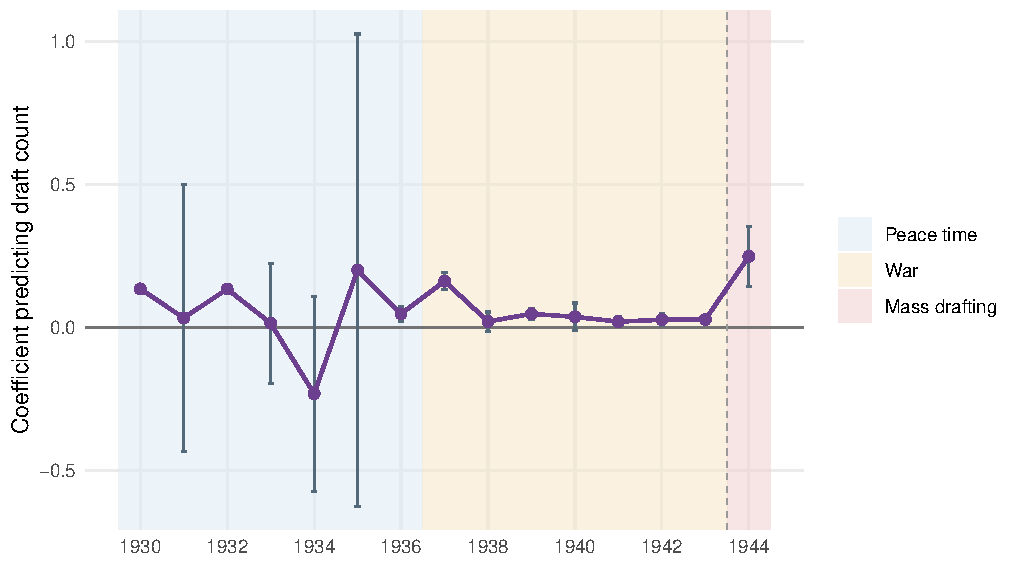
\includegraphics[width=0.84\textwidth]{Results/draft1944_pre_draft_trajectories/draft_intensity_orthogonality_workers.pdf}
    \vspace{1mm}
    \parbox{0.9\textwidth}{\centering\tiny Predictor: workers in team $\times$ occupation cell. Sample: units with at least one 1944 draftee. Dependent variable is 1944 draft count. Conditional on section and position; controls for log cumulative male baseline. Bars show 95\% confidence intervals.}
\end{frame}

\begin{frame}[t]{Draft intensity orthogonality: cell size DID}
    \hypertarget{app:orthogonality-workers-table}{}
    \scriptsize
    \centering
    \begin{threeparttable}
    \begin{tabular}{lcc}
        \toprule
        & Cell + year FE & Section/position + year FE \\
        \midrule
        Workers $\times$ War & -0.000 & -0.003 \\
        & (0.000) & (0.008) \\
        Workers $\times$ Mass drafting & -0.155$^{***}$ & 0.264$^{***}$ \\
        & (0.036) & (0.076) \\
        \midrule
        Observations & 652 & 936 \\
        Cells & \multicolumn{2}{c}{475} \\
        Sections & \multicolumn{2}{c}{173} \\
        Baseline male employment (log) & Yes & Yes \\
        \bottomrule
    \end{tabular}
    \begin{tablenotes}[flushleft]
        \tiny
        \item \textit{Notes:} Dependent variable is 1944 draft count in units with at least one 1944 draftee. Coefficients report whether the listed margin predicts draft intensity differently in war or mass-drafting years relative to peace time. Peace time, 1930--1936, is the omitted period; War is 1937--1943; Mass drafting is 1944. Standard errors clustered by section in parentheses. $^{***}p<0.01$, $^{**}p<0.05$, $^{*}p<0.1$.
    \end{tablenotes}
    \end{threeparttable}
\end{frame}

\begin{frame}[t]{Draft intensity orthogonality: internal flows}
    \hypertarget{app:orthogonality-internal-plot}{}
    \centering
    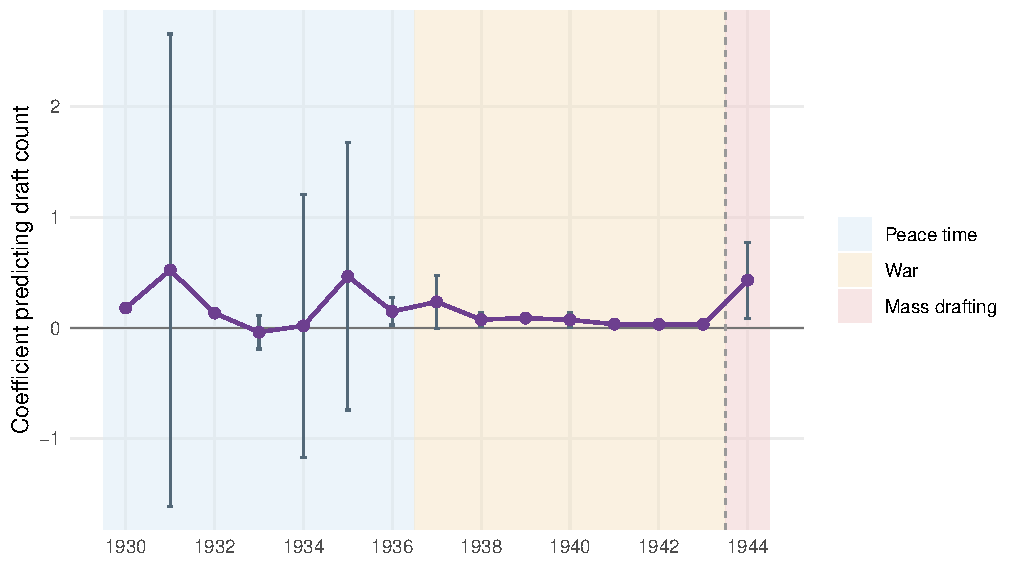
\includegraphics[width=0.84\textwidth]{Results/draft1944_pre_draft_trajectories/draft_intensity_orthogonality_internal.pdf}
    \vspace{1mm}
    \parbox{0.9\textwidth}{\centering\tiny Predictor: total internal arrivals. Sample: units with at least one 1944 draftee. Dependent variable is 1944 draft count. Conditional on section and position; controls for log cumulative male baseline. Bars show 95\% confidence intervals.}
\end{frame}

\begin{frame}[t]{Draft intensity orthogonality: internal flows DID}
    \hypertarget{app:orthogonality-internal-table}{}
    \scriptsize
    \centering
    \begin{threeparttable}
    \begin{tabular}{lcc}
        \toprule
        & Cell + year FE & Section/position + year FE \\
        \midrule
        Total internal $\times$ War & 0.000 & 0.008 \\
        & (0.000) & (0.020) \\
        Total internal $\times$ Mass drafting & -3.972$^{***}$ & 0.313$^{**}$ \\
        & (1.444) & (0.143) \\
        \midrule
        Observations & 652 & 936 \\
        Cells & \multicolumn{2}{c}{475} \\
        Sections & \multicolumn{2}{c}{173} \\
        Baseline male employment (log) & Yes & Yes \\
        \bottomrule
    \end{tabular}
    \begin{tablenotes}[flushleft]
        \tiny
        \item \textit{Notes:} Dependent variable is 1944 draft count in units with at least one 1944 draftee. Coefficients report whether the listed margin predicts draft intensity differently in war or mass-drafting years relative to peace time. Peace time, 1930--1936, is the omitted period; War is 1937--1943; Mass drafting is 1944. Standard errors clustered by section in parentheses. $^{***}p<0.01$, $^{**}p<0.05$, $^{*}p<0.1$.
    \end{tablenotes}
    \end{threeparttable}
\end{frame}

\begin{frame}[t]{Draft intensity orthogonality: retention}
    \hypertarget{app:orthogonality-retention-plot}{}
    \centering
    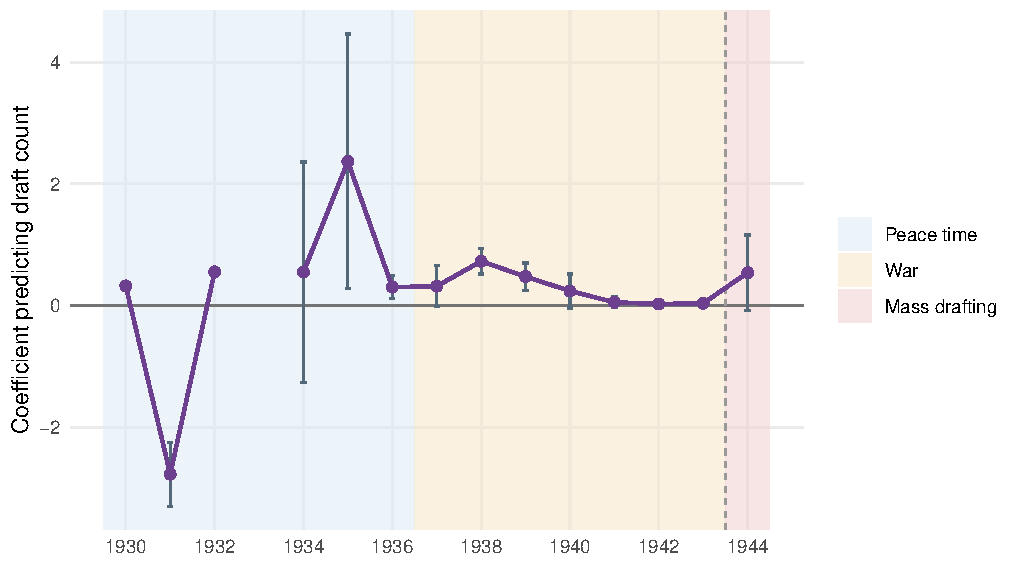
\includegraphics[width=0.84\textwidth]{Results/draft1944_pre_draft_trajectories/draft_intensity_orthogonality_retention.pdf}
    \vspace{1mm}
    \parbox{0.9\textwidth}{\centering\tiny Predictor: same-section retention. Sample: units with at least one 1944 draftee. Dependent variable is 1944 draft count. Conditional on section and position; controls for log cumulative male baseline. Bars show 95\% confidence intervals.}
\end{frame}

\begin{frame}[t]{Draft intensity orthogonality: retention DID}
    \hypertarget{app:orthogonality-retention-table}{}
    \scriptsize
    \centering
    \begin{threeparttable}
    \begin{tabular}{lcc}
        \toprule
        & Cell + year FE & Section/position + year FE \\
        \midrule
        Retention $\times$ War & -0.001$^{**}$ & -0.074 \\
        & (0.000) & (0.058) \\
        Retention $\times$ Mass drafting & -3.971$^{***}$ & 0.307 \\
        & (1.444) & (0.268) \\
        \midrule
        Observations & 652 & 936 \\
        Cells & \multicolumn{2}{c}{475} \\
        Sections & \multicolumn{2}{c}{173} \\
        Baseline male employment (log) & Yes & Yes \\
        \bottomrule
    \end{tabular}
    \begin{tablenotes}[flushleft]
        \tiny
        \item \textit{Notes:} Dependent variable is 1944 draft count in units with at least one 1944 draftee. Coefficients report whether the listed margin predicts draft intensity differently in war or mass-drafting years relative to peace time. Peace time, 1930--1936, is the omitted period; War is 1937--1943; Mass drafting is 1944. Standard errors clustered by section in parentheses. $^{***}p<0.01$, $^{**}p<0.05$, $^{*}p<0.1$.
    \end{tablenotes}
    \end{threeparttable}
\end{frame}

\begin{frame}[t]{Draft intensity orthogonality: same-dept transfers}
    \hypertarget{app:orthogonality-same-dept-plot}{}
    \centering
    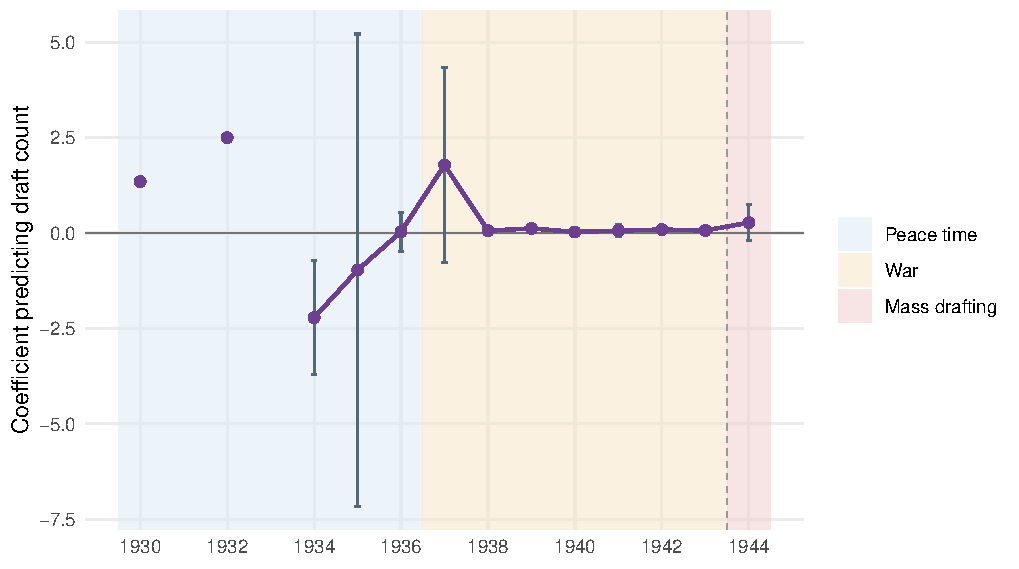
\includegraphics[width=0.84\textwidth]{Results/draft1944_pre_draft_trajectories/draft_intensity_orthogonality_same_dept.pdf}
    \vspace{1mm}
    \parbox{0.9\textwidth}{\centering\tiny Predictor: cross-section transfers within department. Sample: units with at least one 1944 draftee. Dependent variable is 1944 draft count. Conditional on section and position; controls for log cumulative male baseline. Bars show 95\% confidence intervals.}
\end{frame}

\begin{frame}[t]{Draft intensity orthogonality: same-dept transfers DID}
    \hypertarget{app:orthogonality-same-dept-table}{}
    \scriptsize
    \centering
    \begin{threeparttable}
    \begin{tabular}{lcc}
        \toprule
        & Cell + year FE & Section/position + year FE \\
        \midrule
        Same dept. $\times$ War & 0.000 & 0.024 \\
        & (0.000) & (0.031) \\
        Same dept. $\times$ Mass drafting & NA & 0.236 \\
        & NA & (0.235) \\
        \midrule
        Observations & 652 & 936 \\
        Cells & \multicolumn{2}{c}{475} \\
        Sections & \multicolumn{2}{c}{173} \\
        Baseline male employment (log) & Yes & Yes \\
        \bottomrule
    \end{tabular}
    \begin{tablenotes}[flushleft]
        \tiny
        \item \textit{Notes:} Dependent variable is 1944 draft count in units with at least one 1944 draftee. Coefficients report whether the listed margin predicts draft intensity differently in war or mass-drafting years relative to peace time. Peace time, 1930--1936, is the omitted period; War is 1937--1943; Mass drafting is 1944. Standard errors clustered by section in parentheses. $^{***}p<0.01$, $^{**}p<0.05$, $^{*}p<0.1$.
    \end{tablenotes}
    \end{threeparttable}
\end{frame}

\begin{frame}[t]{Draft intensity orthogonality: diff.-dept transfers}
    \hypertarget{app:orthogonality-diff-dept-plot}{}
    \centering
    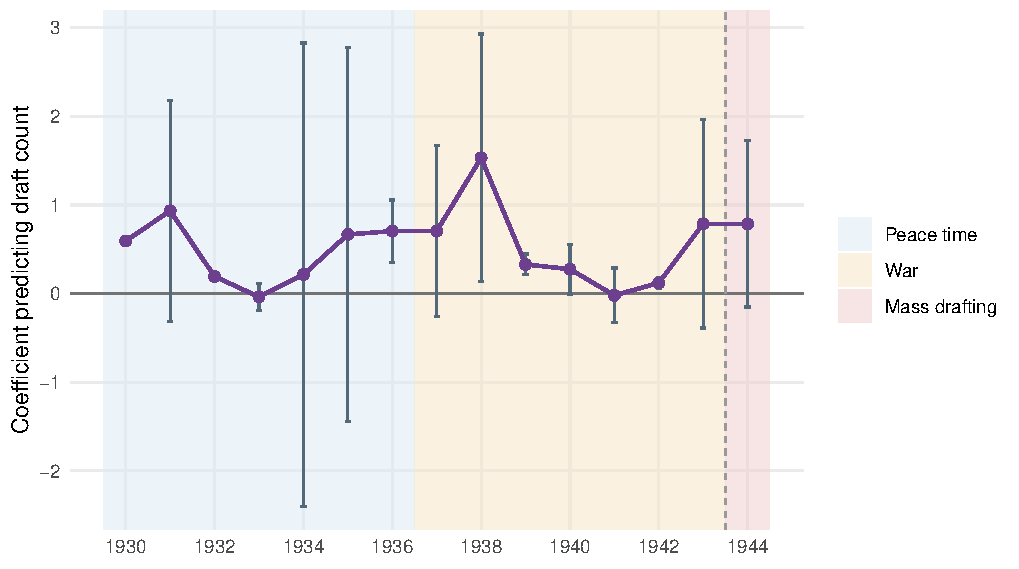
\includegraphics[width=0.84\textwidth]{Results/draft1944_pre_draft_trajectories/draft_intensity_orthogonality_diff_dept.pdf}
    \vspace{1mm}
    \parbox{0.9\textwidth}{\centering\tiny Predictor: cross-department transfers. Sample: units with at least one 1944 draftee. Dependent variable is 1944 draft count. Conditional on section and position; controls for log cumulative male baseline. Bars show 95\% confidence intervals.}
\end{frame}

\begin{frame}[t]{Draft intensity orthogonality: diff.-dept transfers DID}
    \hypertarget{app:orthogonality-diff-dept-table}{}
    \scriptsize
    \centering
    \begin{threeparttable}
    \begin{tabular}{lcc}
        \toprule
        & Cell + year FE & Section/position + year FE \\
        \midrule
        Diff. dept. $\times$ War & -0.000 & 0.110$^{**}$ \\
        & (0.001) & (0.049) \\
        Diff. dept. $\times$ Mass drafting & NA & 0.664$^{*}$ \\
        & NA & (0.397) \\
        \midrule
        Observations & 652 & 936 \\
        Cells & \multicolumn{2}{c}{475} \\
        Sections & \multicolumn{2}{c}{173} \\
        Baseline male employment (log) & Yes & Yes \\
        \bottomrule
    \end{tabular}
    \begin{tablenotes}[flushleft]
        \tiny
        \item \textit{Notes:} Dependent variable is 1944 draft count in units with at least one 1944 draftee. Coefficients report whether the listed margin predicts draft intensity differently in war or mass-drafting years relative to peace time. Peace time, 1930--1936, is the omitted period; War is 1937--1943; Mass drafting is 1944. Standard errors clustered by section in parentheses. $^{***}p<0.01$, $^{**}p<0.05$, $^{*}p<0.1$.
    \end{tablenotes}
    \end{threeparttable}
\end{frame}

\begin{frame}[t]{Draft intensity orthogonality: new hires}
    \hypertarget{app:orthogonality-new-hires-plot}{}
    \centering
    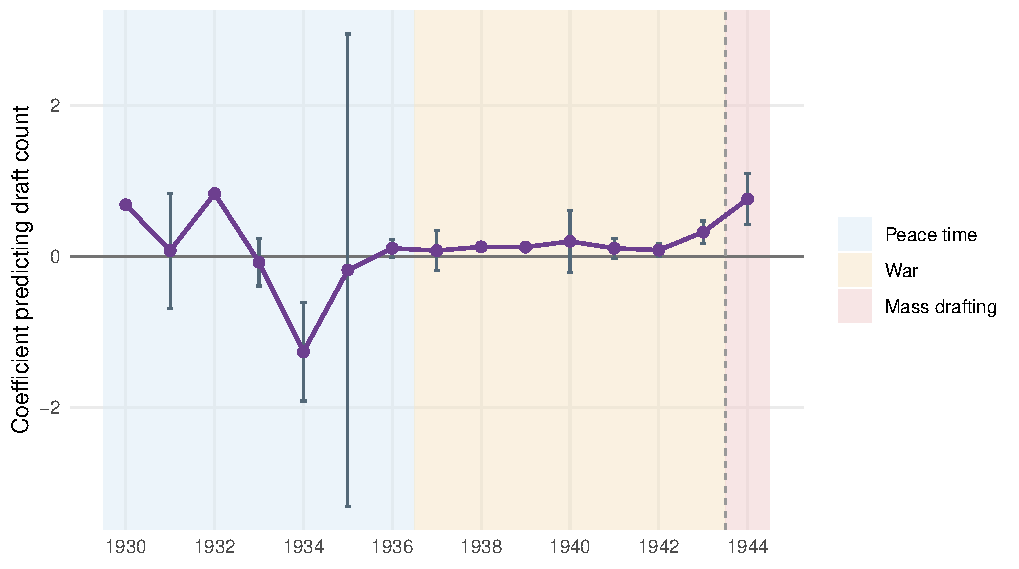
\includegraphics[width=0.84\textwidth]{Results/draft1944_pre_draft_trajectories/draft_intensity_orthogonality_new_hires.pdf}
    \vspace{1mm}
    \parbox{0.9\textwidth}{\centering\tiny Predictor: external new hires. Sample: units with at least one 1944 draftee. Dependent variable is 1944 draft count. Conditional on section and position; controls for log cumulative male baseline. Bars show 95\% confidence intervals.}
\end{frame}

\begin{frame}[t]{Draft intensity orthogonality: new hires DID}
    \hypertarget{app:orthogonality-new-hires-table}{}
    \scriptsize
    \centering
    \begin{threeparttable}
    \begin{tabular}{lcc}
        \toprule
        & Cell + year FE & Section/position + year FE \\
        \midrule
        New hires $\times$ War & 0.001 & -0.001 \\
        & (0.001) & (0.033) \\
        New hires $\times$ Mass drafting & -0.777$^{***}$ & 0.727$^{***}$ \\
        & (0.252) & (0.212) \\
        \midrule
        Observations & 652 & 936 \\
        Cells & \multicolumn{2}{c}{475} \\
        Sections & \multicolumn{2}{c}{173} \\
        Baseline male employment (log) & Yes & Yes \\
        \bottomrule
    \end{tabular}
    \begin{tablenotes}[flushleft]
        \tiny
        \item \textit{Notes:} Dependent variable is 1944 draft count in units with at least one 1944 draftee. Coefficients report whether the listed margin predicts draft intensity differently in war or mass-drafting years relative to peace time. Peace time, 1930--1936, is the omitted period; War is 1937--1943; Mass drafting is 1944. Standard errors clustered by section in parentheses. $^{***}p<0.01$, $^{**}p<0.05$, $^{*}p<0.1$.
    \end{tablenotes}
    \end{threeparttable}
\end{frame}

